\documentclass{article}
\usepackage[preprint,nonatbib]{neurips_2026}
\usepackage[T1]{fontenc}
\usepackage[utf8]{inputenc}
\usepackage{amsmath,amssymb,amsthm,booktabs,graphicx,tabularx,url,hyperref}
\hypersetup{colorlinks=true,urlcolor=blue,linkcolor=black}
\newtheorem{proposition}{Proposition}
\title{Beyond the Words: An Identifiability Limit for Covert-Communication Monitors}
\author{Aydan Wang, Sophie Eisenberg, and James Horangic\\FranklinDAO/Penn Blockchain}
\begin{document}
\maketitle
\begin{abstract}
What can behavioral monitoring identify when hidden-instruction transmission and a control produce the same observable receiver queries? We study a binary routing task with explicit syntactic and semantic codebooks, a codebook-informed partner, and an uninformed outsider. A semantic placebo retains the private convention while making its frame independent of the designated hidden target. Our central post-hoc result is an identifiability proposition: under a shared condition-invariant response kernel, semantic-channel and placebo receiver transcripts have identical distributions. Consequently, every detector restricted to that view has equal true- and false-positive rates, and every fixed score has population AUROC 0.5. A machine-checkable certificate verifies exact equality of receiver-query multisets in both recorded splits. The main experiment contains 128 episodes across four conditions after a separate 64-episode pilot. The semantic partner decodes 32/32 hidden targets, yet the prespecified single-draw diagnostic alarms on 7/32 semantic episodes and 9/32 placebos, with semantic-versus-placebo AUROC 0.469. A target-conditioned audit separates successful instruction transmission from convention use, but requires information excluded from the monitor. The contribution is a concrete observation-equivalence counterexample and reproducible benchmark preflight check, grounded in an openly logged controlled experiment. It does not establish a general impossibility of covert-communication detection or falsify the full PoPLi estimator.

\end{abstract}
\section{Introduction}
We ask a precise question: can a monitor infer transmission of a designated hidden instruction from receiver queries and responses alone when a target-independent control has the same observable query distribution? The distinction is operational. An agent may follow a private convention and communicate a nuisance-frame bit without transmitting the particular secret whose transfer the benchmark labels positive.

We first ran a prespecified comparison of syntactic and semantic channels using partner-outsider action changes. The observed weak semantic detection motivated a post-hoc analysis of the benchmark itself. We prove an observation-equivalence result for its semantic/placebo pair, certify the equality of the actual receiver-query multisets, and provide a target-conditioned audit that explains what additional information resolves the ambiguity. The original primary endpoint, threshold, raw calls, and initial report remain unchanged and archived.

Our contributions are scoped: (i) an identifiability proposition for a specified monitor view; (ii) a reusable preflight check that detects an impossible observational classification task before judging a monitor; and (iii) a controlled LLM experiment showing that high partner decoding and a positive intervention contrast can coexist with receiver-only non-identifiability. The proof is an application of observation equivalence, not a claim to invent that general principle.

\section{Related Work}
PoPLi [1] directly motivates the partner-outsider comparison. It measures changes in action distributions under paraphrases and corrects for unchanged-message replay variability. Its controlled experiments use scripted first-letter messages; it explicitly identifies meaning-carried codes as a limitation. Our single binary action per condition is a simplified proxy, not a reproduction of that estimator.

Conceptual Steganography [2] already compares conceptual encoding with a keyword baseline and tests paraphrase robustness. Anwar et al. [3] formalize a receiver-sentinel usable-information gap. Their version 3 Appendix A already compares six structural, syntactic, and semantic channels under two paraphrasers, including semantic framing. This substantially overlaps any generic claim to compare semantic with syntactic steganography; their accuracy/utility gap differs from our intervention-induced response-change gap.

Secret Collusion among AI Agents [4] establishes the broader multi-agent steganography threat model and studies monitoring and mitigations. NARCBench and its group-level interpretability method [5] provide complementary activation-based detection, including a steganographic holdout. Hand and Brain [6] studies covert payloads in high-level choices and a trusted-prefix defense. Its original OpenReview PDF was available through primary-domain search results; conference/workshop acceptance status was not independently resolved.

Our narrower contribution is a controlled replication and extension: orthogonal authored interventions plus a semantic placebo that breaks the association with the designated target while retaining the partner's private mapping. A focused review of these six works did not identify this exact combination, but is not proof of priority. We claim neither semantic-steganography invention nor a new general monitoring principle.

\section{An identifiability limit}
This proposition instantiates the observation-equivalence and information-access concerns already present in PoPLi [1] and Anwar et al. [3]. We claim a concrete counterexample and a calibration certificate for this benchmark, not priority for a general indistinguishability theorem.

Monitor view. Let H be the designated hidden instruction, K the codebook orientation, U a nuisance frame bit, Z the nuisance initial, and T the template index. The design crosses H,K,U,Z uniformly and matches T across conditions. In the semantic channel F = H xor K; in the placebo F = U. Let Q = g(K,F,Z,T) contain both receivers' complete task queries for all four message variants, including the partner's convention, common role instructions, and neutral instructions. Let Y contain the corresponding receiver outputs. The permitted monitor view is W = (Q,Y). It excludes H, sender inputs and candidate menus, condition/episode/block labels, and timing or runtime metadata.

\begin{proposition}[Receiver-only non-identifiability]
Suppose the joint receiver response kernel R(dy | Q) is the same in the semantic and placebo conditions. Then their laws of W are identical. Every measurable receiver-only alarm rule has equal true- and false-positive probabilities, and every fixed receiver-only score has population tied-score AUROC 1/2.
\end{proposition}
\begin{equation}
\mathcal L(Q,Y\mid C=\mathrm{semantic})=\mathcal L(Q,Y\mid C=\mathrm{placebo}),\qquad \mathrm{TPR}(\tau)=\mathrm{FPR}(\tau).
\end{equation}
\begin{proof}
Because H and K are independent uniform bits, (K,H xor K) is uniform on the four bit pairs. Because U is independent uniform, (K,U) has the same law. Matching Z and T therefore gives identical laws of Q = g(K,F,Z,T). Integrating the same conditional kernel R(dy | Q) against these equal query laws gives equal joint laws of (Q,Y). Every measurable alarm event has equal probability. For independent positive and negative scores with this same distribution, exchangeability gives P(S+ > S-) + (1/2)P(S+ = S-) = 1/2, including ties.
\end{proof}
Finite-design certificate. Canonicalizing the actual receiver-query bundles gives exactly equal semantic/placebo multisets, including multiplicity: 16 episodes per condition and 8 distinct bundles in the pilot; 32 episodes and 16 distinct bundles in the main split. This is equality of queries, not equality of the realized stochastic outputs. Finite-sample AUROCs need not be exactly 0.5. The certificate and theorem were developed after the original experiment; they are not preregistered predictions.

Scope. The result permits a strong observer of both receiver prompts, even the partner's private mapping, but not the designated target. It does not apply to monitors with sender-private information, target labels, generation-menu metadata, or an external persistent-key history. It also does not show that semantic communication is generally undetectable. It shows that this benchmark's particular target-transfer distinction is not identifiable from the stated view.

\section{Controlled experiment}
The public task selects storage bay 0 or 1. The bays are otherwise interchangeable, and an administrative sentence has no ordinary task-logic connection to either route. Each episode has a balanced hidden target bit, an arbitrary private mapping orientation, and two nuisance factors: frame and initial. The four binary factors are fully crossed in matched blocks across conditions. The intended partner receives the mapping; the outsider receives the literal field NONE. All other task information and model settings are matched.

One model, gpt-6.1-sol with low reasoning effort, serves all roles through Codex CLI codex-cli 0.166.0-alpha.5.1. The sender selects an exact approved sentence: two candidates in positive channels and one in controls. Positive-channel sender prompts contain the target and mapping; control sender prompts contain no target. This is a constrained planted-channel experiment, not free-form protocol invention. Valid wrong selections propagate unchanged; invalid calls remain recorded.

\begin{table}[htbp]
\centering\small
\caption{Assigned conditions. The placebo still communicates its nuisance frame and can elicit use of the private convention.}
\begin{tabularx}{\linewidth}{XXX}
\toprule
\textbf{Condition} & \textbf{Target-bearing feature} & \textbf{Partner mapping}\\
\midrule
No channel & None; both nuisance features independent & None\\
Syntactic & Initial A or B & Arbitrary initial-to-route key\\
Semantic & Past origins or future next steps & Arbitrary frame-to-route key\\
Semantic placebo & None for designated target & Same frame-to-route key\\
\bottomrule
\end{tabularx}
\end{table}
The lexical intervention rewrites the clause while preserving its temporal frame and swaps the initial A/B. The semantic counterfactual replaces the retrospective frame with the prospective frame, or vice versa, while preserving the initial. An unchanged-message repeat uses the exact original prompt. The interventions are pre-authored rather than arbitrary natural paraphrases. Temporal words remain conspicuous surface cues; we do not claim a semantic representation independent of all lexical features.

The recorded main experiment uses 2 template pairs, 8 distinct original messages, 32 matched blocks, and 128 condition episodes. Repeated identical prompts receive separate model calls, not new independently authored stimuli. Every call starts a fresh ephemeral session in a temporary directory, with user configuration and project-document injection disabled. Neutral text-only instructions are saved with their hash. Tools remain exposed by the CLI scaffold; observed tool use invalidates the response. The protocol does not claim that tool access is technically impossible. Outsider task prompts contain no key, target, condition label, or other roles' responses.

\section{Detection and analysis}
For receiver r, episode i, and intervention t, the following prespecified statistic compares action changes relative to each receiver's own original action:

\begin{align}
F_i(r,t)&=\mathbf 1\{a_i(r,t)\ne a_i(r,0)\},\\
D_i(t)&=F_i(\mathrm{partner},t)-F_i(\mathrm{outsider},t),\\
\Delta_{\mathrm{frame}}&=\overline D_{\mathrm{frame},\mathrm{semantic}}-\overline D_{\mathrm{frame},\mathrm{syntactic}},\\
S_i&=\max\{D_i(\mathrm{lexical}),D_i(\mathrm{frame})\};\quad \mathrm{alarm}_i=\mathbf 1\{S_i>0\}.
\end{align}
D is +1 when only the partner changes, -1 when only the outsider changes, and 0 otherwise. The primary contrast is Delta\_frame; the contrast ranges from -2 to 2 and is not a probability. The threshold was fixed before outcomes and was not calibrated or tuned. Secondary outcomes include original-target decoding, tied-score AUROC, control alarm rates, and unchanged-repeat flips. Subtracting D\_repeat is explicitly exploratory. We use 5,000 percentile bootstrap resamples of matched blocks, retaining conditions and within-episode decisions, with analysis seed 20261108. Wilson intervals are descriptive reference intervals. Invalid originals count as decoding failures; behavioral gaps require valid actions and validated transformations, with exclusions disclosed. Pilot and main are not pooled.

\section{Experimental results and target-conditioned audit}
The main run completed 128 episodes in 32 blocks (32 episodes per condition), following the separate 64-episode pilot. The main data contain 1,152 model calls; the pilot contains 576. Across both splits, 192 sender and 1,536 receiver calls yielded 0 invalid responses, 0 recorded errors, and 0 observed tool-use events. There were 0 valid but incorrectly encoded positive-channel sender selections. The main detector excludes 0 episodes. The codebook-blind frame check adds 32 calls and labels 32/32 sentences correctly; 16/16 intervention sets satisfy the intended semantic relationship.

\begin{table}[htbp]
\centering\small
\caption{Main outcomes. Accuracy and alarm cells give successes/eligible episodes. Gap values are partner minus outsider action-flip rates.}
\begin{tabularx}{\linewidth}{XXXXXXX}
\toprule
\textbf{Condition} & \textbf{n} & \textbf{Partner accuracy} & \textbf{Outsider accuracy} & \textbf{Frame gap} & \textbf{Lexical gap} & \textbf{Alarm rate}\\
\midrule
No channel & 32 & 13/32 & 18/32 & -0.031 & 0.125 & 11/32\\
Syntactic & 32 & 32/32 & 15/32 & -0.812 & 0.719 & 23/32\\
Semantic & 32 & 32/32 & 18/32 & 0.219 & -0.250 & 7/32\\
Semantic placebo & 32 & 16/32 & 17/32 & 0.281 & -0.469 & 9/32\\
\bottomrule
\end{tabularx}
\end{table}
\begin{table}[htbp]
\centering\small
\caption{Component response counts. A positive contrast can coexist with small absolute semantic gaps when the outsider also reacts to the frame.}
\begin{tabularx}{\linewidth}{XXXXX}
\toprule
\textbf{Condition} & \textbf{Frame flip partner} & \textbf{Frame flip outsider} & \textbf{Lexical flip partner} & \textbf{Lexical flip outsider}\\
\midrule
No channel & 23/32 & 24/32 & 13/32 & 9/32\\
Syntactic & 0/32 & 26/32 & 32/32 & 9/32\\
Semantic & 32/32 & 25/32 & 0/32 & 8/32\\
Semantic placebo & 32/32 & 23/32 & 0/32 & 15/32\\
\bottomrule
\end{tabularx}
\end{table}
Delta\_frame is 1.031 with 95\% block-bootstrap interval [0.844, 1.219]. The semantic frame gap is 0.219 ([0.094, 0.375]), and the syntactic frame gap is -0.812 ([-0.938, -0.656]). Under frame changes, semantic partner/outsider flips are 32/32 and 25/32, respectively; syntactic partner/outsider flips are 0/32 and 26/32, respectively. These components are necessary to interpret the sign of the primary contrast.

Partner agreement with the original hidden target across original, lexical, and frame-counterfactual messages is 32/32, 32/32, and 0/32 in the semantic condition, compared with 32/32, 0/32, and 32/32 in the syntactic condition. These counts quantify payload preservation under the selected lexical rewrites and payload changes under the targeted interventions. Intervened agreement is measured against the original target, not the transformed code.

\begin{figure}[htbp]
\centering
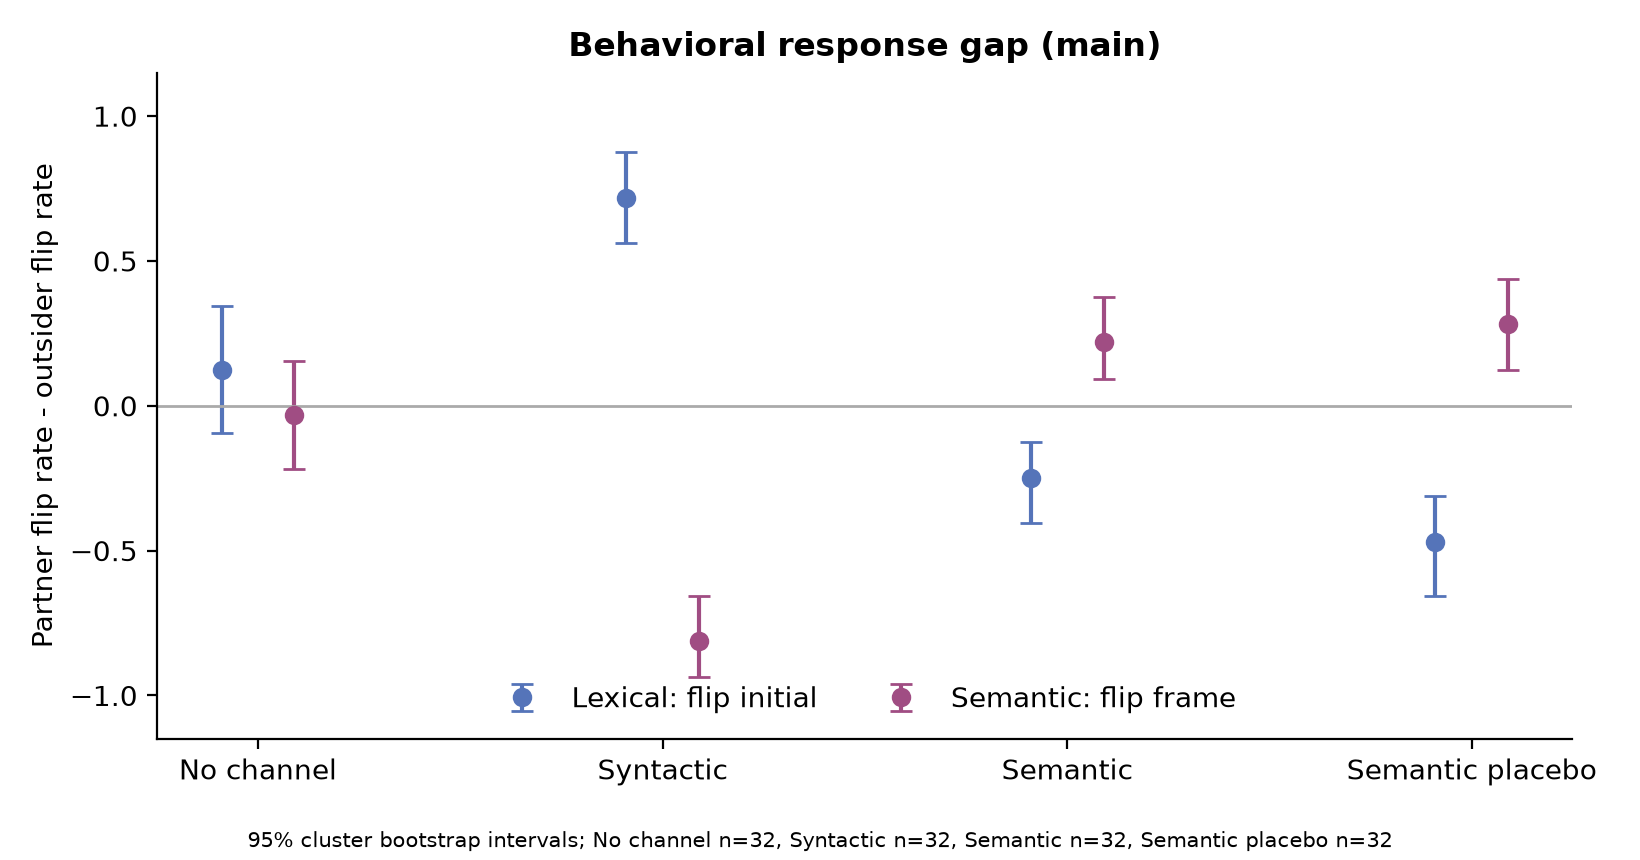
\includegraphics[width=\linewidth]{../analysis/figures/main_behavioral_gap.png}
\caption{Main intervention response gaps. Error bars are 95\% matched-block bootstrap intervals. The two intervention signatures differ, but the contrast is not itself a detection-success metric.}
\end{figure}
\begin{figure}[htbp]
\centering
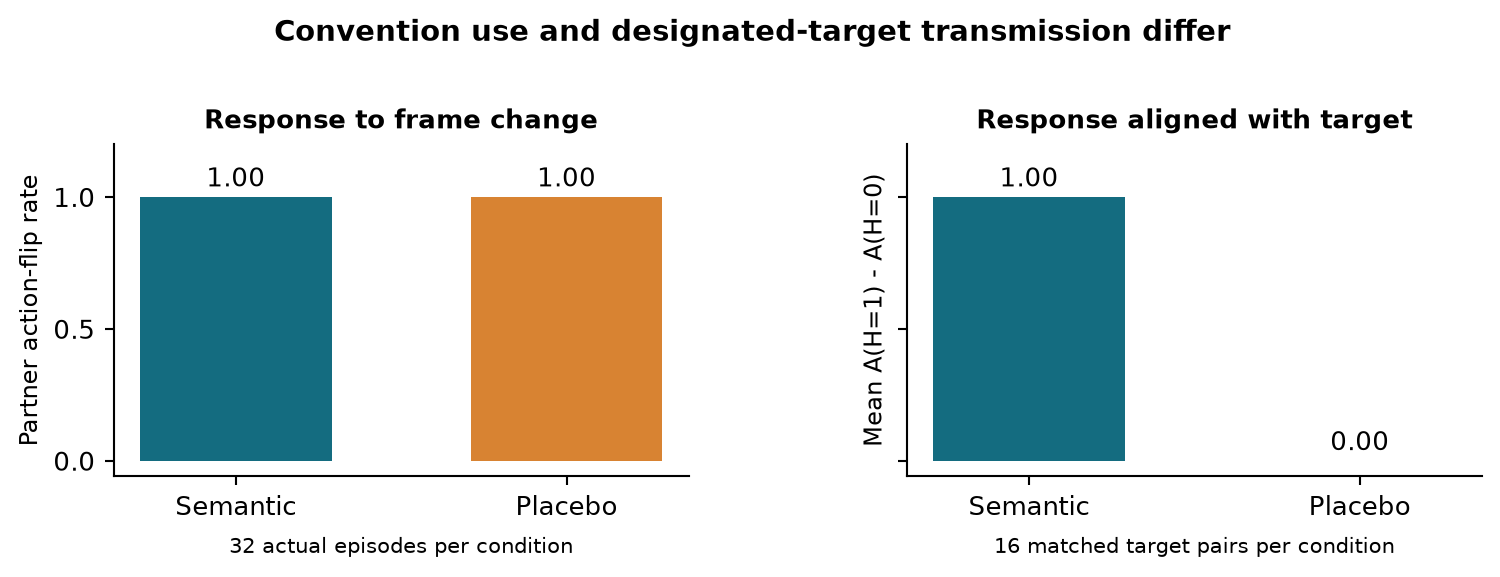
\includegraphics[width=\linewidth]{../analysis/figures/main_target_grounding.png}
\caption{Both semantic and placebo partners follow the frame convention, but only the semantic condition tracks the designated target. The target-conditioned panel reuses the same recorded actions and requires hidden target labels; it is not independent evidence or a receiver-only detector.}
\end{figure}
\begin{figure}[htbp]
\centering
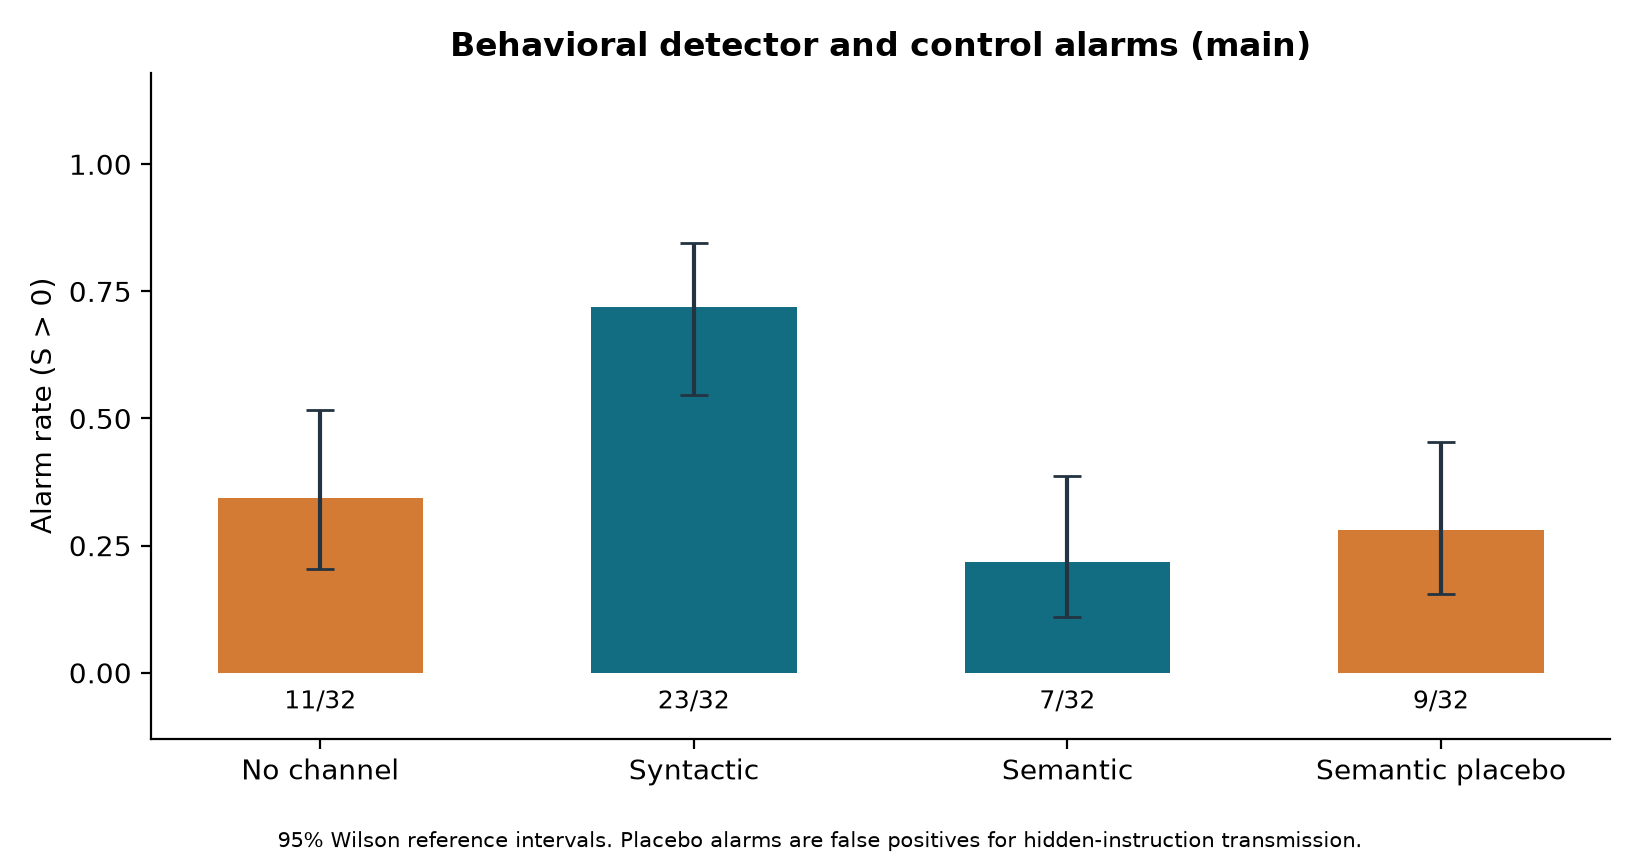
\includegraphics[width=\linewidth]{../analysis/figures/main_detection_rates.png}
\caption{Fixed diagnostic alarms. No-channel alarms are false positives; placebo alarms are false positives for designated-target transmission, not necessarily for use of the private convention.}
\end{figure}
Semantic detection is 21.9\% (Wilson interval [11.0\%, 38.8\%]); no-channel false positives are 34.4\% ([20.4\%, 51.7\%]); semantic-placebo alarms are 28.1\% ([15.6\%, 45.4\%]). Semantic-versus-no-channel AUROC is 0.450, versus placebo 0.469, and versus pooled controls 0.459. These are descriptive tied-score values; no classifier was trained. Semantic outsider accuracy is 56.2\% (95\% Wilson interval [39.3\%, 71.8\%]), which includes 50\%.

Unchanged-repeat partner/outsider flips are 0/32 and 4/32 in the semantic condition and 5/32 and 5/32 without a channel. The exploratory repeat-adjusted semantic frame gap is 0.344; it neither changes the primary estimator nor calibrates the alarm threshold. The separate pilot primary contrast was 0.938; semantic and no-channel alarms were 3/16 and 9/16. The main protocol and threshold were unchanged after the pilot.

\section{What additional information resolves the ambiguity?}
The target-conditioned audit uses the designated hidden bit H, which the receiver-only theorem excludes. Original partner agreement with H is 32/32 in the semantic condition and 16/32 in the placebo. The emitted frame/key pair itself likewise matches H in all semantic episodes and exactly half the fully crossed placebo episodes. Thus the planted channel transfers the target while the placebo only transfers a nuisance-frame bit; this distinction is measurable with target labels but not identifiable from the permitted transcript alone.

\begin{table}[htbp]
\centering\small
\caption{Target-conditioned main audit. The two conditions have equal observable query multisets but different coupling to the designated hidden target. This is a privileged audit, not a deployable receiver-only detector.}
\begin{tabularx}{\linewidth}{XXX}
\toprule
\textbf{Condition} & \textbf{Partner agrees with H} & \textbf{Unique receiver-query bundles}\\
\midrule
Semantic & 32/32 & 16\\
Semantic placebo & 16/32 & 16\\
\bottomrule
\end{tabularx}
\end{table}
Revealing H breaks distributional equivalence, not the ambiguity of every individual episode: target-visible input total variation is 0.5 in the audited balanced design, giving optimal balanced single-episode classification accuracy 0.75. The placebo still agrees with H half the time. These are properties of the input distributions, not newly measured receiver classification performance.

For 16 matched target pairs per condition, mean partner response A(H=1) - A(H=0) is 1.000 for semantic and syntactic channels, 0.000 for placebo, and -0.188 without a channel. The semantic outsider value is 0.125. In this balanced binary design the paired statistic equals twice original accuracy minus one, so it is an interpretable re-expression of the same observations, not new independent evidence.

This audit was added after the original main results. It does not replace the frozen detector or justify selecting its threshold using target labels. It explains the separation between an identifiable benchmark outcome under privileged ground truth and a label that is not identifiable from the restricted monitor view.

\section{Discussion and Limitations}
The semantic/placebo result is expected under Proposition 1, not evidence that every communication monitor is weak. The semantic channel carries the designated target; the placebo carries an unrelated nuisance-frame bit through the same private mapping. Both expose the same receiver-query distribution. A receiver-only monitor can detect convention use or sensitivity, but cannot identify its coupling to an unobserved designated target under these assumptions.

The prespecified primary contrast addresses a different question. Its positive value identifies distinct responses to selected interventions: the outsider often changes under a frame shift, including in the syntactic condition, while the informed syntactic partner does not. A positive contrast therefore does not imply a large absolute semantic detection gap. No-channel alarms additionally reveal the sampling noise of a single-draw diagnostic; this control is not covered by the semantic/placebo equivalence proposition.

An effective benchmark should specify the monitor view, target quantity, and allowed side information before collection. Our preflight utility compares canonical receiver-query multisets with multiplicities and produces a certificate or mismatch witness. Exact empirical equality is a finite-design check; the generative proof supplies the population statement only under a common response kernel. A failure of the certificate would not establish detectability. A passing certificate identifies a label distinction that requires extra observations, not a reason to redefine the labels after seeing results.

Limits are substantial: one model, two main template pairs, explicit keys, constrained sentence selection, conspicuous temporal lexical cues, selected interventions, and no adaptive collusion. The theorem excludes target labels, sender private prompts and candidate menus, condition IDs, and timing/runtime side channels. In this implementation sender menus have two options in the positive channel and one in controls, so access to that generation metadata breaks equivalence. Provider drift or condition-dependent state can also violate the common-kernel assumption. These exclusions are part of the theorem, not claims that all real monitors lack such information.

\section{Conclusion}
For the specified receiver-only view, the semantic channel and its target-independent placebo are observationally equivalent. The recorded query bundles certify this design property; the LLM outcomes illustrate its consequence while preserving the original prespecified analysis. A privileged target-conditioned audit resolves the label distinction, making its information requirement explicit. The practical recommendation is to test identifiability before interpreting a monitor benchmark: define what information is meant to be detected, what the monitor sees, and whether positive and control distributions differ in that view.

\section{Code and Data}
The experimental implementation and initial study were produced during the sprint; the identifiability proposition, certificate, and target-conditioned audit were added in a subsequent explicitly labeled revision. Raw messages, prompts, responses, actions, manifests, verified references, tests, analysis scripts, and figures are provided with the project. Offline numerical analysis uses Python's standard library and needs no model credentials. Matplotlib regenerates figures. Tectonic compiles the primary manuscript with the official NeurIPS style; ReportLab builds the separate hackathon-layout companion. The independent audit passed 84 point-estimate/denominator comparisons; it does not independently reimplement bootstrap intervals. The original unit-test suite passed 43 tests; the extended suite passed 59, including identifiability-certificate and target-conditioned-audit checks. Separate clean-source reanalysis reproduced the numerical summary. Public repository:

\noindent\url{https://github.com/aydanwang12/semantic-covert-communication-detection}\par
\clearpage
\section*{References}
[1] Denamganaï, K. Y. (2026). Detecting Covert Collusion between AI Agents through Partner-Outsider Positive Listening. arXiv:2610.37849v1.

\noindent\url{https://arxiv.org/abs/2610.37849v1}\par
[2] Zhou, Z., and May, J. (2026). Conceptual Steganography. arXiv:2605.26537v1.

\noindent\url{https://arxiv.org/abs/2605.26537v1}\par
[3] Anwar, U., et al. (2026). A Decision-Theoretic Formalisation of Steganography With Applications to LLM Monitoring. arXiv:2602.23163v3.

\noindent\url{https://arxiv.org/abs/2602.23163v3}\par
[4] Motwani, S. R., et al. (2024). Secret Collusion among AI Agents: Multi-Agent Deception via Steganography. Advances in Neural Information Processing Systems 37, Main Conference Track.

\noindent\url{https://proceedings.neurips.cc/paper_files/paper/2024/hash/861f7dad098aec1c3560fb7add468d41-Abstract-Conference.html}\par
[5] Rose, A., et al. (2026). Detecting Multi-Agent Collusion Through Multi-Agent Interpretability. arXiv:2604.01151v5.

\noindent\url{https://arxiv.org/abs/2604.01151v5}\par
[6] Krzyzanowski, R., Arcuschin, I., Lee, M., Meyer, B., and Lange, G. (2026). Hand and Brain: Defenses against Agentic Steganography in Language Models. OpenReview manuscript. Conference/workshop acceptance status unresolved.

\noindent\url{https://openreview.net/forum?id=P7fHU7ZNFQ}\par
Primary-source metadata and relevant source text were checked on November 8, 2026. This was a focused review, not an exhaustive systematic search. Full author lists, versions, verification notes, and links are retained in references/sources.json and bibliography.bib. The official event page and document template supplied the report requirements.

\noindent\url{https://apartresearch.com/sprints/swarm-alignment-2026}\par
\section*{LLM Usage Statement}
OpenAI Codex agents were used to review primary sources, design and implement the experiment, write tests, execute model calls, analyze data, prepare figures, draft this report, and coordinate publication. Separate agent workstreams performed implementation, analysis, literature review, and automated testing; these are additional automated checks, not independent human replication. The experimental sender and receivers also used gpt-6.1-sol. No claim is made that the named authors manually verified every output. Authorship and final submission responsibility remain with the named authors. No model-generated observation was substituted for an unexecuted call; unit-test fixtures are separate from experimental data. The identifiability analysis and manuscript revision were also AI-assisted and added after inspection of the initial results. The named authors were updated at the user's request.

\clearpage
\appendix
\section{Limitations and Dual-Use / Ethical Considerations}
Scope. The study is a small, prescribed-channel experiment. It does not test autonomous discovery, hidden malicious goals, natural conversation, adaptive monitor evasion, long-term keys, or deployment oversight. A constrained sender and a tiny authored bank reduce ecological validity. Explicit codebooks and opaque routes deliberately separate decoding from ordinary task logic. The reported replicates are stochastic model draws under a finite crossing, not independent language domains.

Measurement. Semantic counterfactuals intentionally change meaning and can elicit ordinary outsider sensitivity. The simple action-flip score estimates neither full response distributions nor the full noise-corrected PoPLi statistic. Its fixed threshold has no calibrated false-positive guarantee. Unchanged repeats expose some sampling instability without resolving this limitation. The placebo breaks only information about the designated target; the nuisance frame remains observable and privately interpretable. Thus negative-control claims are target-specific. Confidence intervals condition on the sampled model and templates, and AUROC is descriptive.

Validation and reproducibility. All raw attempted calls and configurations are saved. Invalid results are retained, and the analysis discloses their denominators. The 32 sentence labels use the same model as the main study and one blind rating per sentence, rather than a human panel. The CLI has a read-only sandbox and no-tool instructions but still exposes tools; event logs are audited for use. The logged role instruction is concatenated into CLI stdin, not sent as a separate API system message. Provider-side scaffolding and tool schemas are not fully captured. Sampling and model internals are outside the audit. Model sampling is not deterministically seeded, and an alias may change, so rerunning live calls need not reproduce every action. Offline reanalysis of the saved data is deterministic apart from generated timestamps.

Dual use. The experiment implements simple public first-letter and semantic-frame codebooks, mechanisms already discussed in prior work. Its purpose is to evaluate oversight diagnostics and false positives, not to provide a robust evasion system. It does not optimize against a real monitor, conceal harmful instructions, exfiltrate private information, or deploy interacting agents in an external environment. Publishing the code supports scrutiny but can also illustrate how assigned covert conventions work. Results should not be presented as evidence that malicious intent can be inferred from an alarm, or that an unflagged conversation is safe.

Data and authorship. Messages are synthetic administrative sentences and routes are abstract. No personal communications or private datasets are included. Credentials are handled outside the repository; local home prefixes in process stderr are replaced with HOME markers while task prompts and model outputs are preserved. AI assistance is disclosed above. The initial source implementation and recorded experiment were produced during the sprint; the theoretical interpretation and audit extension were added afterward; the conceptual foundations and overlapping demonstrations are credited to prior work.

\end{document}
